\documentclass[[12pt,twoside]{book}
\usepackage{_my_document_style}
\begin{document}
\begin{figure}[t]%[H]%[!htbp]
  \centering
  %\checkoddpage
  %\centering
    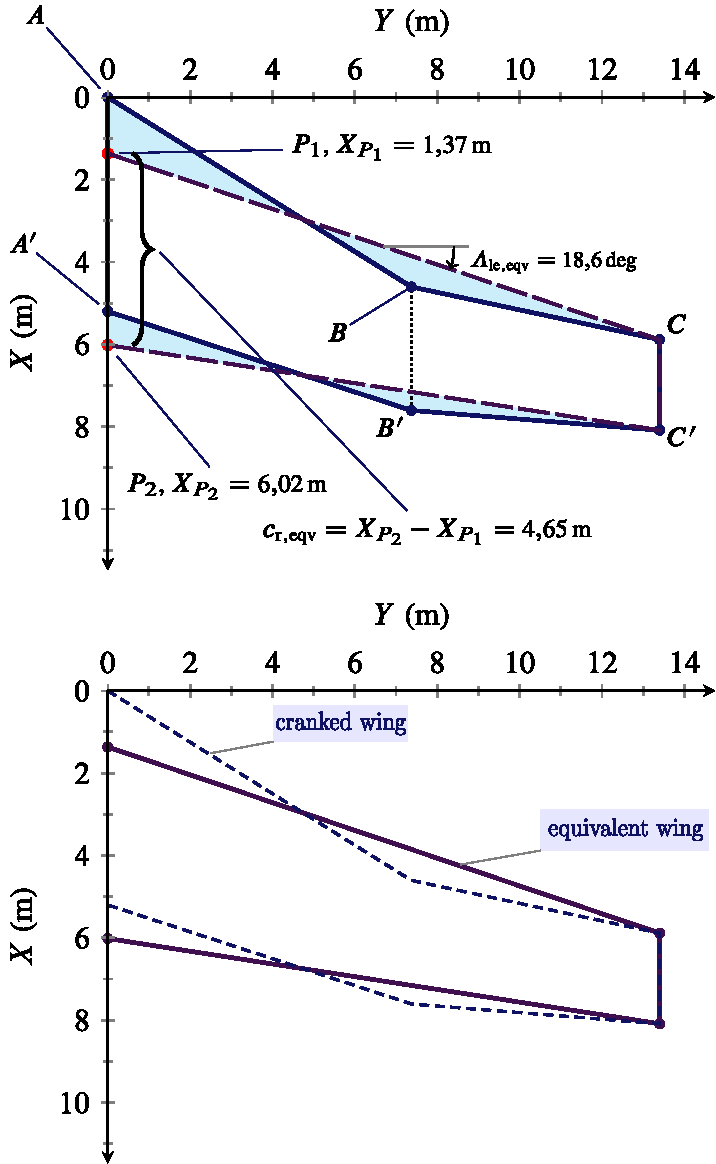
\includegraphics[width=0.68\textwidth]{Chapter_2/equivalent_plan_form_of_a_cranked_wing/wing_planform_basic_3_drawing.pdf}
  \caption{\finalhyphendemerits=1000
           Equivalent planform of the wing assigned in the exercises  \ref{example:Equivalent:Plan:Form:Of:A:Cranked:Wing} and \ref{example:Geometric:Characteristics:Of:A:Cranked:Wing}.
  }
  \label{fig:Cranked:Wing:Planform:Results:B}%
\end{figure}
%
\def\mySpanWingMT{26.800000}
\def\mySpanWingIMT{14.740000}
\def\mySpanWingIIMT{12.060000}
\def\myRootChordWingLongitudinalPlaneMT{4.650000}
\def\myChordRootWingIMT{5.200000}
\def\myChordRootWingIIMT{3.000000}
\def\myChordTipWingMT{2.200000}
\def\myChordTipWingIMT{3.000000}
\def\myChordTipWingIIMT{2.200000}
\def\mySweepLEWingIDEG{32.000000}
\def\mySweepLEWingIIDEG{12.000000}
\def\mySweepLEWingIRAD{0.558505}
\def\mySweepLEWingIIRAD{0.209440}
\def\myEquivalentSweepLEWingRAD{18.639942}
\def\myEquivalentSweepLEWingDEG{0.325328}
\def\myXEquivalentChordLEToApexWingMT{1.370000}
\def\myXEquivalentChordTEToApexWingMT{6.020000}
\def\myEquivalentTaperRatioWing{0.473118}

%
\begin{myExampleX}{Equivalent planform of a cranked wing}{\ding{46}}% \ \Keyboard\ %
\label{example:Equivalent:Plan:Form:Of:A:Cranked:Wing}
%
\noindent
With reference to the example~\ref{example:Geometric:Characteristics:Of:A:Cranked:Wing} and to
figure~\ref{fig:Cranked:Wing}
we want to find a simple planform,
with straight leading and trailing edges, which is equivalent to a wing \emph{cranked} with two panels.
The equivalent wing has area $S$ of the planform, wingspan $b$ and tip chord $c_\mathrm{t}$ 
equal to those of the wing \emph{cranked}.
In particular, from the diagram of the figure~\ref{fig:Cranked:Wing}
the relative position of the tip chord with respect to the apex $A$ of the assigned wing
is unchanged. For  the given \emph{cranked} wing in the example ~\ref{example:Geometric:Characteristics:Of:A:Cranked:Wing} we want to know:

\adjustbox{center=\textwidth}
{%
$P_1$\,, $P_2$\,, $c_{\mathrm{r,eqv}}$\,, $\lambda_{\mathrm{eqv}}$\,, $\Lambda_{\mathrm{le,eqv}}$
}
% \,, $Y_{\bar{c}}$

\medskip
The positions $P_1$ and $P_2$, respectively, of the edge of leading edge and trailing edge of the equivalent wing must be found by duly imposing
the conditions of equivalence stated above.
The location of the point $P_1$ is calculated by imposing:
\[
\text{Area}\big(P_1 C C' P_3 P_1\big) = \text{Area}\big(A B C C' P_3 A \big)
\]
or, said $C''$ the projection of $C$ on the axis of $X$, imposing:
\[
\text{Area}\big(P_1 C C'' P_1\big) = \text{Area}\big(A B C C'' A \big)
\]
The location of the point $P_2$ is calculated by imposing:
\[
\text{Area}\big(P_2 C' P_3 P_2\big)=\text{Area}\big(A' B' C' P_3 A' \big)
\]
From the reference scheme, the data of the problem allow to calculate
\[
Y_B = \frac{b_1}{2} = \mathunderline{mydarkblue}{
  \calcSI[round-precision=2,fixed-exponent=0,scientific-notation=fixed]{0.5*\mySpanWingIMT}{\metre}
}
\]

\[
X_B = Y_B \tan \Lambda_{\mathrm{le},1}
  = \calcSI[round-precision=2,fixed-exponent=0,scientific-notation=fixed]{0.5*\mySpanWingIMT}{\metre}
    \cdot \tan( \SI[round-precision=3]{\mySweepLEWingIRAD}{\radian} )
  = \mathunderline{mydarkblue}{
    \calcSI[round-precision=2,fixed-exponent=0,scientific-notation=fixed]{
      0.5*\mySpanWingIMT * tan(\mySweepLEWingIRAD)
    }{\metre}
  }
\]

\[
Y_C = \frac{b}{2} 
  = \mathunderline{mydarkblue}{
    \calcSI[round-precision=2,fixed-exponent=0,scientific-notation=fixed]{0.5*\mySpanWingMT}{\metre}
  }
\]

\[
X_C = X_B + \frac{b_2}{2} \tan \Lambda_{\mathrm{le},2} =
  \calcSI[round-precision=2,fixed-exponent=0,scientific-notation=fixed]{
    0.5*\mySpanWingIMT * tan(\mySweepLEWingIRAD)
  }{\metre}
  +
  \calcSI[round-precision=2,fixed-exponent=0,scientific-notation=fixed]{
    0.5*\mySpanWingIIMT
  }{\metre}
  \cdot \tan( \SI[round-precision=3]{\mySweepLEWingIIRAD}{\radian} )
  = \mathunderline{mydarkblue}{
    \calcSI[round-precision=2,fixed-exponent=0,scientific-notation=fixed]{
      0.5*\mySpanWingIMT * tan(\mySweepLEWingIRAD)
      + 0.5*\mySpanWingIIMT * tan(\mySweepLEWingIIRAD)
    }{\metre}
  }
\]

\[
Y_{C'} = Y_{C}
  = \mathunderline{mydarkblue}{
    \calcSI[round-precision=2,fixed-exponent=0,scientific-notation=fixed]{0.5*\mySpanWingMT}{\metre}
  }
\]

\[
X_{C'} = X_C + c_{\mathrm{t}}
  = \calcSI[round-precision=2,fixed-exponent=0,scientific-notation=fixed]{
    0.5*\mySpanWingIMT * tan(\mySweepLEWingIRAD)
    + 0.5*\mySpanWingIIMT * tan(\mySweepLEWingIIRAD)
  }{\metre}
  + \SI[round-precision=2]{\myChordTipWingMT}{\metre}
  = \mathunderline{mydarkblue}{
    \calcSI[round-precision=2,fixed-exponent=0,scientific-notation=fixed]{
      0.5*\mySpanWingIMT * tan(\mySweepLEWingIRAD)
      + 0.5*\mySpanWingIIMT * tan(\mySweepLEWingIIRAD)
      + \myChordTipWingMT
    }{\metre}
  }
\]

\[
Y_{B'} = Y_{B}
  = \mathunderline{mydarkblue}{
    \calcSI[round-precision=2,fixed-exponent=0,scientific-notation=fixed]{0.5*\mySpanWingIMT}{\metre}
  }
\]

\[
X_{B'} = X_{B} + c_{\mathrm{t},1}
  = \calcSI[round-precision=2,fixed-exponent=0,scientific-notation=fixed]{
    0.5*\mySpanWingIMT * tan(\mySweepLEWingIRAD)
  }{\metre}
  + \SI[round-precision=2]{\myChordTipWingIMT}{\metre}
  = \mathunderline{mydarkblue}{
    \calcSI[round-precision=2,fixed-exponent=0,scientific-notation=fixed]{
      0.5*\mySpanWingIMT * tan(\mySweepLEWingIRAD)
      + \myChordTipWingIMT
    }{\metre}
  }
\]

\[
X_{A'} = c_{\mathrm{r},1}
  = \mathunderline{mydarkblue}{
    \SI[round-precision=2]{\myChordRootWingIMT}{\metre}
  }
\]

The condition that defines the point $P_1$  becomes
\[
\frac{1}{2}\big( X_C - X_{P_1} \big) \, Y_C
  = \frac{1}{2} \Big[ X_C + \big( X_C - X_B \big) \Big] \, Y_B
    + \frac{1}{2}\big( X_C - X_B \big) \big( Y_C - Y_B \big)
\]
that is, an algebraic equation in the unknown $X_{P_1}$. Replacing the values previously
calculated, we get
\[
X_{P_1}
  = \mathunderline{mydarkblue}{
    \SI[round-precision=2]{\myXEquivalentChordLEToApexWingMT}{\metre}
  }
\]

Similarly, the condition that defines the point $P_2$ becomes
\[
\frac{1}{2}\big( X_{C'} - X_{P_2} \big) \, Y_{C'}
  = \frac{1}{2} \Big[ \big( X_{C'} - X_{A'} \big) + \big( X_{C'} - X_{B'} \big) \Big] \, Y_{B'}
    + \frac{1}{2}\big( X_{C'} - X_{B'} \big) \big( Y_{C'} - Y_{B'} \big)
\]
that is, an algebraic equation in the unknown $X_{P_2}$. Replacing the values previously
calculated, we get
\[
X_{P_2}
  = \mathunderline{mydarkblue}{
    \SI[round-precision=2]{\myXEquivalentChordTEToApexWingMT}{\metre}
  }
\]

The previous results allow to calculate the root chord of the equivalent wing
\[
c_{\mathrm{r,eqv}} = X_{P_2} - X_{P_1}
  = \SI[round-precision=2]{\myXEquivalentChordTEToApexWingMT}{\metre}
    - \SI[round-precision=2]{\myXEquivalentChordLEToApexWingMT}{\metre}
  = \mathunderline{mydarkblue}{
    \SI[round-precision=2]{\myRootChordWingLongitudinalPlaneMT}{\metre}
  }
\]
From this data it is possible to obtain the taper ratio:
\[
\lambda_{\mathrm{eqv}} = \frac{c_\mathrm{t}}{c_{\mathrm{r,eqv}}}
  = \frac{
      \SI[round-precision=2]{\myChordTipWingMT}{\metre}
    }{ 
      \SI[round-precision=2]{\myRootChordWingLongitudinalPlaneMT}{\metre}
    }
  = \mathunderline{mydarkblue}{
    \SI[round-precision=2]{\myEquivalentTaperRatioWing}{}
  }
\]
that is a value different from that of the original wing
$\lambda = c_\mathrm{t}/c_{\mathrm{r},1}=\SI[round-precision=2]{\myTaperRatioWing}{}$.

Find a simple planform that is equivalent to a planform wing broken edges is useful when semiempirical methods are to be used for evaluation of the aerodynamic coefficients of an aircraft. In some cases, these methods require data for a simple wing---
for example the arrow angle $\Lambda_{\mathrm{le}}$ or $\Lambda_{c/4}$ ---
and, having a \emph{cranked} wing, it is appropiate to identifie angles as
$\Lambda_{\mathrm{le,eqv}}$ or $\Lambda_{c/4,\mathrm{eqv}}$
of the equivalent wing before using them for the required calculation.
The sweep angle of the leading edge of the equivalent wing is calculated as follows:
\[
\tan \Lambda_{\mathrm{le,eqv}} = \frac{X_C - X_{P_1}}{b/2}
  = \frac{
    \calcSI[round-precision=2,fixed-exponent=0,scientific-notation=fixed]{
      0.5*\mySpanWingIMT * tan(\mySweepLEWingIRAD)
      + 0.5*\mySpanWingIIMT * tan(\mySweepLEWingIIRAD)
    }{\metre}
      - \SI[round-precision=2]{\myXEquivalentChordLEToApexWingMT}{\metre}
  }{ 
    \calcSI[round-precision=2,fixed-exponent=0,scientific-notation=fixed]{0.5*\mySpanWingMT}{\metre}
  }
\quad \Rightarrow \quad
\Lambda_{\mathrm{le,eqv}}
  = \mathunderline{mydarkblue}{
    \SI[round-precision=3]{\myEquivalentSweepLEWingRAD}{\radian}
  }
  = \mathunderline{mydarkblue}{
    \SI[round-precision=1]{\myEquivalentSweepLEWingDEG}{\deg}
  }
\] 
\end{myExampleX}
\begin{figure}[t]%[H]%[!htbp]
%  %\centering
\checkoddpage
%  %\centering
  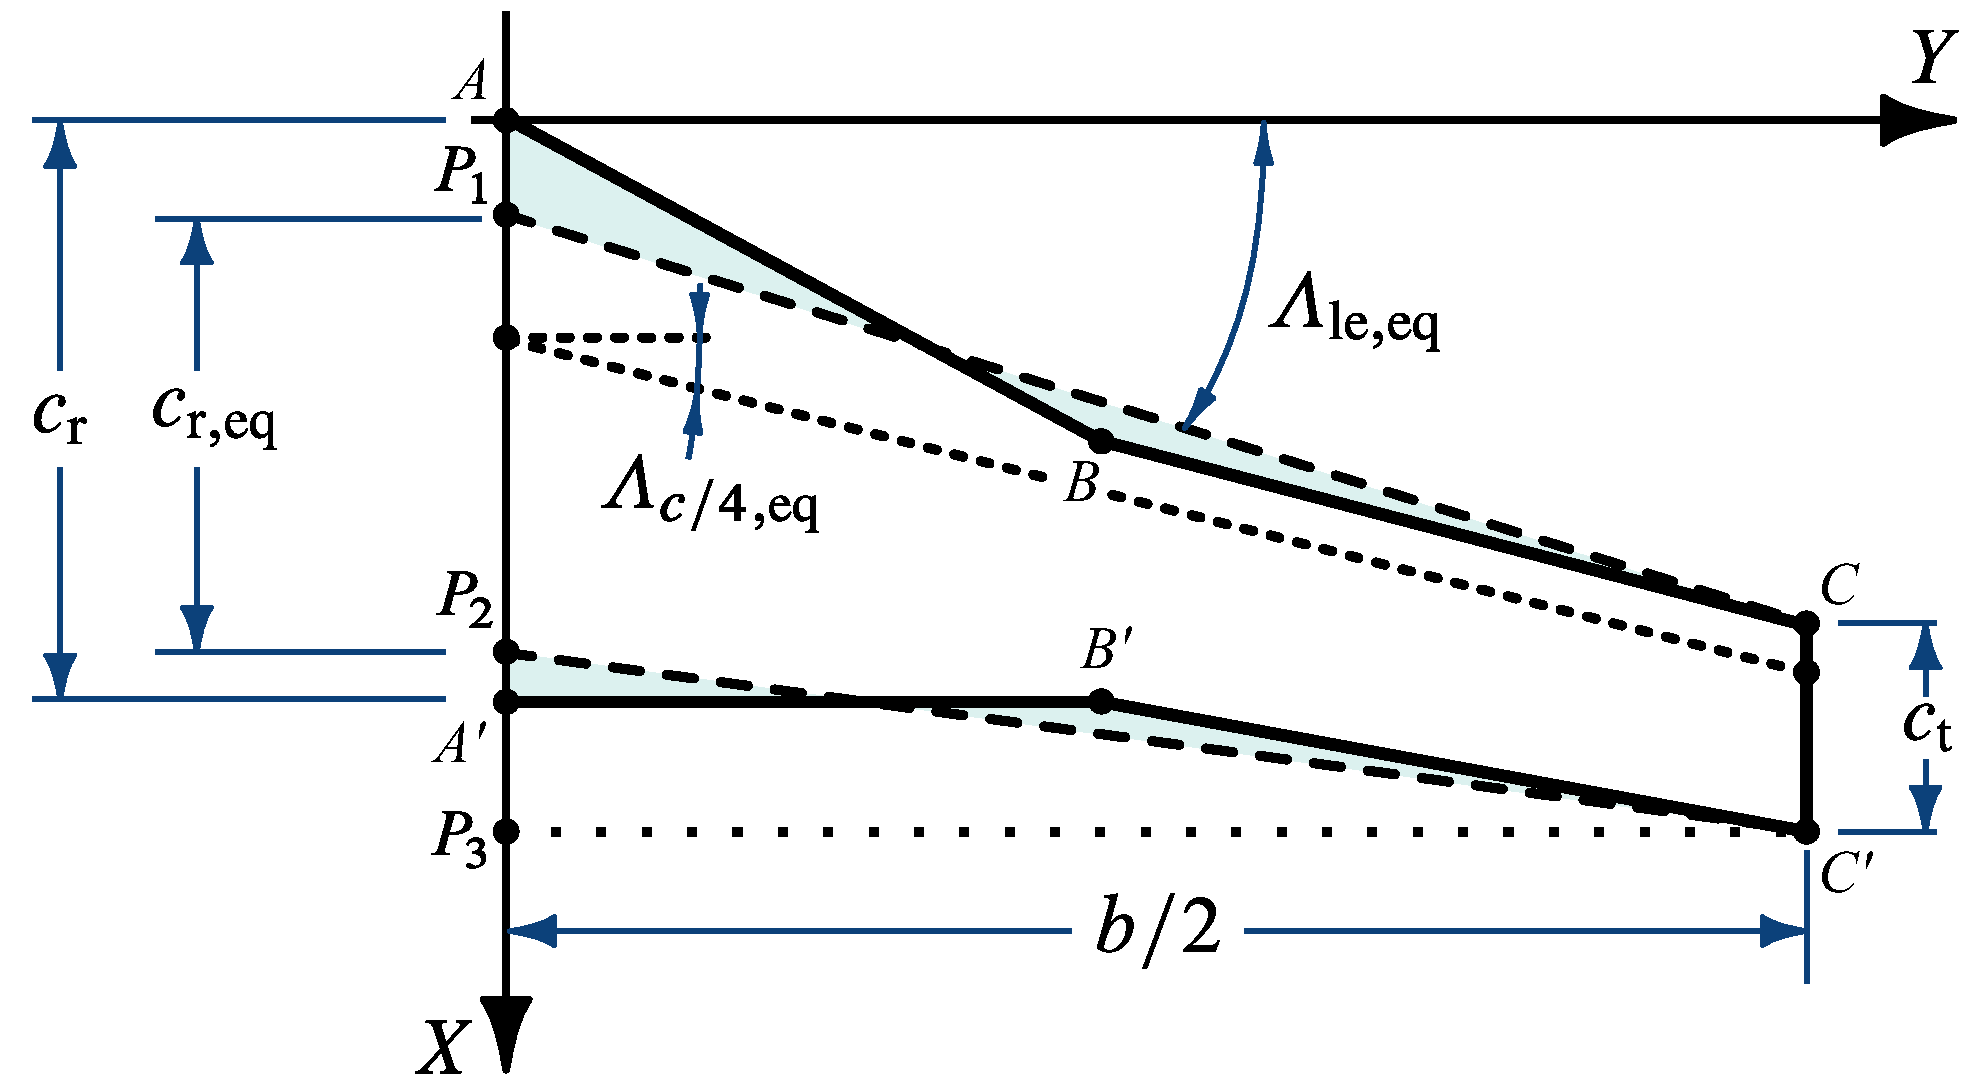
\includegraphics[width=0.78\textwidth]{Chapter_2/equivalent_plan_form_of_a_cranked_wing/equivalent_wing.pdf}
  \caption{\finalhyphendemerits=1000
         Wing with leading and trailing edges not straight and equivalent wing with straight edges.}
 \label{fig:Equivalent:Wing:Planform:Defs}%
\end{figure}
\end{document} 
